\section{System Architecure}
\label{sec:systemarch}

This section presents the core elements of the Morpheus system and its 
role in the \textit{automated question answering} process. 

\subsection{Query Processing}
\label{sec:query_processing}
  
The \emph{Query Resolution Recorder} or QRR is an instrumented web browser
used to track the search pathways to an answer for a \textit{guide user's} query. It
also helps the guide user to identify categories (optional) for the query terms. 
Morpheus has two types of categories: \emph{intput categories} and \emph{output categories}.
Input categories annotates the query terms into a class or category, which are 
useful in finding similar queries. On the other hand, output categories give hints
to the expected answer of a user query. Morpheus captures all
this query information in the representation of an SSQ. For example, suppose, a guide user
tries to answer the query ``A 1997 Toyota Camry V6 needs what size tires?'', using
Morpheus. With the help of the QRR, she may choose relevant query terms and assign
\emph{input categories} to them: Toyota : manufacturer, Camry V6 : 
model, tire : automotive parts, and size as the \emph{output category}. 
In addition, she can log the search pathways to an answer (e.g. P215/60R16)
to this query and select the query \emph{realm} as automotive.      


The \emph{Query Resolution Method} or QRM is a data structure that models the
question answering process. A QRM is usually constructed by a \emph{guide user} with
the help of the QRR. Each QRM contains an \emph{ontological realm}, an SSQ, and
information to support the query answering process. QRMs are associated with an
ontology that has a particular realm i.e. an ontological realm. In addition, 
the QRM contains information required to visit each page needed to 
answer the query as well as the order of visitation. For each
dyanamic page, it stores the list of inputs to the URL such as form inputs and
the possible referrence outputs (highlighted portions of the web page).


% NLP arch. 
% Joir-dan

A \textit{regular user} query is parsed into specific terms by an \textit{NLP
engine} using some linguistic techniques [Need to be completed]. The SSQ generated by the NLP
Engine contains user query and parsed terms. 


\subsection{Morpheus Ontology and Corpora} 
\label{sec:ontology_corpora}

Morpheus requires a realm-based ontology that contains categories of a
particular realm of interest. For example, the realm-ontology \textit{Automotive}
contains categories that are relevant to the \textit{automotive} realm. In
addition, every leaf node in the category ontology is associated with a corpus of words
that belongs to that category. 

For ontology construction Morpheus uses the Wikipedia pages, categories,
and the WordNet synset heterarchy. This approch is motivated from
YAGO\cite{Suchanek2009phd}. For a given realm, we first find a mapping category 
from the DBpedia categories\cite{Auer07dbpedia:a} (these are extracted from 
the Wikipedia pages). Then we grab all the neighboring categories
using a \textit{Markov Blanket} \cite{PRIS}. In fact, we grab 
the category's parents, its children, and its 
children's other parents using the DBpedia ontology properties \textit{broader}
and \textit{narrower}. Once the blanket is ready, it grabs all parent categories
of the categories in the blanket till it reaches root. Once we have the
categories belongs to a particular domain, we associate them with WordNet synsets
using an algorithm similar to YAGO\cite{Suchanek2009phd}. We determine head noun in the
category name and search for it in the WordNet synsets.
Those Wikipedia categories having no WordNet match are ignored in the our realm
ontology. In fact we uses the WordNet synset heterarchy as the backbone of the   
realm ontology. 

To build a corpus for each of the leaf nodes in the ontology, 
we extract \emph{n-grams} or \emph{terms} from the Wikipedia pages associated with the 
the DBpedia categories \cite{Auer07dbpedia:a}. From this category-term corpora, 
we can find out the likelihood that a term belongs to a particular category, 
which is useful in categorizing the terms in a \emph{regular user's} query [section \ref{sec:qrm_ranking}].    
This likelihood is determined by the probability of a category given a term 
using \textit{Bayes Rule} (Eq. \ref{eq:bayesrule}), since we can 
easily obtain the term-category and term-corpus probabilities as 
relative frequencies. The higher the probability, the more likely a 
term is referring to a category. 

\begin{equation}
\label{eq:bayesrule}
P (category | term) = \frac{P(term | category) P(category)}{P(term)}
\end{equation}    

\subsection{Topic Models and Dcoument Classification }
\label{sec:topicmodels}





\subsection{QRM Ranking Mechanism} 
\label{sec:qrm_ranking}

To answer a regular user's query, a \textit{candidate
SSQ}, Morpheus finds similar SSQs that belong to QRMs the Morpheus data store (a
\textit{qualified SSQ}). We need a similarity measure to match the candidate SSQ
with a qualified SSQ. For the SSQ similarity, we
consider the SSQ components such as query-realm, input
terms and output terms, and their assigned categories or classes. The,
\textit{category divergence} of two categories characteristics their 
similarity based on an ontology class heterarchy. 
It is motivated by the concept of multiple
dispatch in CLOS \cite{Steele1990} and Dylan programming \cite{Barrett1996} for
generic function type matches. 

We use \emph{category divergence} to calculate the relevance between the candiate SSQ
and a qualified SSQ. Each qualified SSQ will
have input terms, output terms, and associated classes, and one realm. For the
candidate SSQ, the relevant category for input terms are determined from the
ontology corpora [section \ref{sec:ontology_corpora}]. The relevance 
of a qualified SSQ to the candidate SSQ is determined by
aggregating the divergence measure of categories associated with them. In addition, 
We order QRMs in the data store in order by descreasing relevance. 
The order provides a ranking for the results to the user. 
The following subsection \ref{sec:ctd} describe \emph{category divergence} in detail.

\subsubsection{Catgeory Divergence}
\label{sec:ctd}

We employ a quasimetric, \textit{category
divergence},
between a source category and a target category using the \textit{topological
structure} of the categories in an ontology. We write $S \prec T$ for the
reflexive
transitive closure of the supercategory relation. Let $d(P,Q)$ represent the hop
distance in the directed ontology inheritance graph from $P$ to $Q$. The
divergence between a source and target category ranges from zero (for identical
categories) to one (for incompatible categories). Let $S$ be the source
category, $T$ be
the target category, and let $C$ be a least common ancestor category of $S$ and
$T$
minimizing $d(S,C) + d(T,C)$. The category divergence between $S$ and $T$ is
defined given by:

\begin{equation}
d_{cat}(S, T) = \begin{cases}
0 & S.{Uri} \equiv T.{Uri}\\
d(S, T)/(3h) & S \prec T\\
1 & T \prec S\\
(d(S,root) + d(S,C) \\ \ \ \ \ + d(T,C))/(3h) & otherwise
\end{cases}
\end{equation}

\noindent where $h$ is the height of the ontology tree.

Note, if $S \prec T$ and $S \not\prec Q$ then $d_{cat}(S,T) <
d_{cat}(S,Q)$, that is, the divergence of a source category to a target
ancestor category is smaller than the divergence of a source category to any
category that is not an ancestor. This is an important property in
determining the compatibility of category for answering queries.  If a
SSQ answers queries concerning an ancestor category, it is more relevant
that a SSQ that answers queries from any non-ancestral category.

% Algorithm 1: figure  
\begin{figure}[t]
\centering
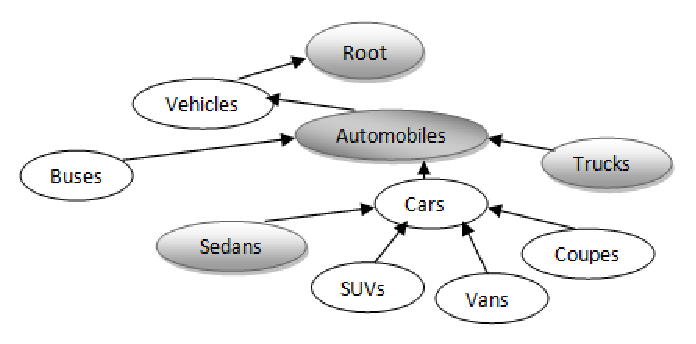
\includegraphics[width=90mm]{img/automotive_ontology.eps}
\caption{An abbreviated graphical representation of an automotive
ontology: This is a manually created ontology, from the Wikipedia category
hierarchy and pages. The edges represent inheritance relationships between the
category in a topology.}
\label{fig:automotive_ontology}
\end{figure}

Suppose we want to find the category divergence between \textit{Toyota Camry}
and \textit{Coupes} [Figure \ref{fig:automotive_ontology}]. 
\textit{Toyota Camry} is the subcategory of \textit{Sedans}, and \textit{Coupes}
is the subcategory of \textit{Cars}. Therefore, the least common ancestor ($C$)
for these two categories is \textit{Cars}. In addition, the tree height is $5$.
So, the normalized divergence $d_{cat}$\textit{(Toyota Camry, Coupes)} is $7/15$
that is calculated from \textit{d(Toyota Camry, Root)} is 5, \textit{d(Toyota
Camry, Cars)} is two, and \textit{d(Coupes, Cars)} is one.


\subsection{Query Resolution Execution} 

Usually, answering a question using the 
deep web requires one to navigate through a sequence of one or 
more web pages. Many of the accesses involve clicks through 
web forms or links to resulting pages. QRM contains the necessary  
information required to re-run this procedure. Once we have 
relevant QRMs through QRM ranking for a given user query, we can  
get answers by re-running the pathways with help of 
the Query Resolution Engine or QRE of Morpheus. 


  


